% VUT FIT MITAI
% MSZ 2021/2022
% Author: Vladimir Dusek
% Login: xdusek27

%%%%%%%%%%%%%%%%%%%%%%%%%%%%%%%%%%%%%%%%%%%%%%%%%%%%%%%%%%%%%%%%%%%%%%%%%%%%%%%%

% Path to figures
\graphicspath{{wap/bezpecnost_webovych_aplikaci/figures}}

%%%%%%%%%%%%%%%%%%%%%%%%%%%%%%%%%%%%%%%%%%%%%%%%%%%%%%%%%%%%%%%%%%%%%%%%%%%%%%%%

\chapter{WAP~--~Bezpečnost webových aplikací (SOP, XSS, CSRF, bezpečnostní hlavičky HTTP).}

%%%%%%%%%%%%%%%%%%%%%%%%%%%%%%%%%%%%%%%%%%%%%%%%%%%%%%%%%%%%%%%%%%%%%%%%%%%%%%%%

\section{Zdroje}

\begin{compactitem}
    \item \path{WAP10_Bezpecnost.pdf}
    \item \path{WAP_2021-04-15.mp4}
\end{compactitem}

%%%%%%%%%%%%%%%%%%%%%%%%%%%%%%%%%%%%%%%%%%%%%%%%%%%%%%%%%%%%%%%%%%%%%%%%%%%%%%%%

\section{Úvod a kontext}

\begin{compactitem}
    \item Pouhé načtení webové stránky znamená vykonání cizího (Javascript) kódu v počítači.

    \item Výrobci prohlížečů vyvažují dva cíle: \begin{compactitem}
        \item Tvorba API umožňujících přístup k HW a SW uživatelského počítače (grafická karta, geolokace, mikrofon, kamera, \ldots).

        \item Zamezení/omezení dopadů škodlivého kódu (ochrana soukromí, úprava dat, podvody, \ldots).
    \end{compactitem}
\end{compactitem}

%%%%%%%%%%%%%%%%%%%%%%%%%%%%%%%%%%%%%%%%%%%%%%%%%%%%%%%%%%%%%%%%%%%%%%%%%%%%%%%%

\section{Same-origin policy (SOP)}

\begin{compactitem}
    \item Origin (původ), definovaný trojicí URI segemntů ---- schéma, doména, port.

    \item Podle této zásady webový prohlížeč povolí skriptům obsaženým na první webové stránce přístup k datům na druhé webové stránce, ale pouze v případě, že obě webové stránky mají stejný origin.

    \item Tato zásada zabraňuje tomu, aby škodlivý skript na jedné stránce získal přístup k citlivým datům na jiné webové stránce prostřednictvím jejího DOM.

    \item \todo{todo}

\end{compactitem}

%%%%%%%%%%%%%%%%%%%%%%%%%%%%%%%%%%%%%%%%%%%%%%%%%%%%%%%%%%%%%%%%%%%%%%%%%%%%%%%%

\section{Cross-site scripting (XSS)}

\begin{compactitem}
    \item Útočník vloží značky nebo skripty do cílové stránky. \begin{compactitem}
        \item Kód se vykoná, když uživatel navštíví stránku.
    \end{compactitem}

    \item Stránka je zranitelná pokud: \begin{compactitem}
        \item Zobrazuje obsah na základě uživatelských vstupů, které jsou bez dostatečné validace.
    \end{compactitem}

    \begin{figure}[H]
        \centering
        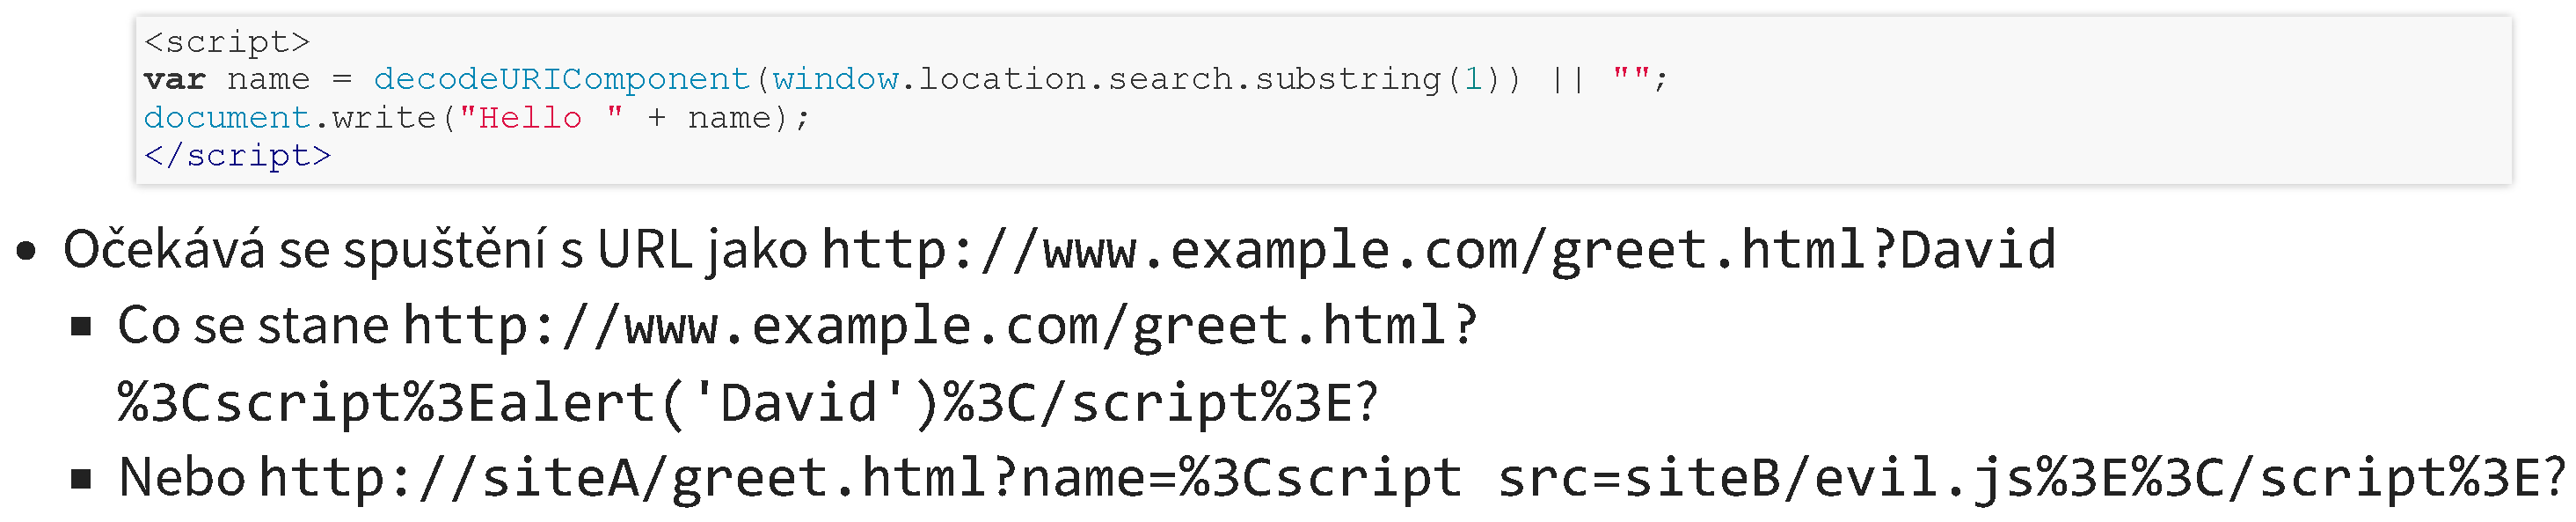
\includegraphics[width=1\linewidth]{xss_priklad.pdf}
        \caption{Příklad XSS.}
    \end{figure}

    \item Varianty XSS: \begin{compactitem}
        \item Trvalé (perzistentní), uložené v databázi.
        \item Dočasné.
        \item Lokální (DOM based)
    \end{compactitem}

    \item Jak realizovat? \begin{compactitem}
        \item Zkracovače odkazů, přesměrování (hlavička Location), znaky kódované pomocí reprezentace ASCII, \ldots
    \end{compactitem}

    \item Nebezpečí XSS: odcizení cookies, obsah web storage, zmáčknuté klávesy, pohyb myši, upravovat formuláře, těžba kryptoměn.

    \item Řešení: \begin{compactitem}
        \item sanitizace vstupů;

        \item HTTP hlavička \textbf{Content Security Policy}: \begin{compactitem}
            \item Zakázání prohlížeči stahování zdrojů mimo povolené origin.
            \item CSP poskytuje majitelům webových stránek standardní metodu pro deklarování schváleného původu obsahu, který by měly prohlížeče na dané webové stránce povolit načítat.
        \end{compactitem}

        \item HTTP hlavička \textbf{Feature policy}: \begin{compactitem}
            \item Stránka vyžaduje, nebo nevyžaduje určité vlastnosti (např. zobrazení na fullscreen, přístup k poloze \ldots).
            \item Omezení přístupu Javascriptu k browser API (např. zakázání přístupu k poloze).
        \end{compactitem}
    \end{compactitem}
\end{compactitem}

%%%%%%%%%%%%%%%%%%%%%%%%%%%%%%%%%%%%%%%%%%%%%%%%%%%%%%%%%%%%%%%%%%%%%%%%%%%%%%%%

\section{Cross-site request forgery (CSRF)}

\begin{compactitem}
    \item \todo{todo}
\end{compactitem}

%%%%%%%%%%%%%%%%%%%%%%%%%%%%%%%%%%%%%%%%%%%%%%%%%%%%%%%%%%%%%%%%%%%%%%%%%%%%%%%%

\section{Bezpečnostní hlavičky HTTP}

\begin{compactitem}
    \item Pomocí bezpečnostních HTTP hlaviček můžeme nastavit různá pravidla pro komunikaci mezi webovým prohlížečem a serverem.

    \item Typicky umožňují povolit nebo zakázat určité funkce prohlížeče pro vyšší bezpečnost a soukromí.

    \item Např. Content Security Policy, Feature Policy, Strict-Transport-Security, X-Frame-Options.
\end{compactitem}

\subsection{HTTPS stripping}

\begin{compactitem}
    \item Man in the middle útok.
    \item Postup: \begin{compactenum}
        \item Uživatel vynechá schéma URI, např. www.example.com.
        \item Výchozí schéma je http.
        \item Útočník nepropaguje přesměrování na HTTPS.
    \end{compactenum}

    \begin{figure}[H]
        \centering
        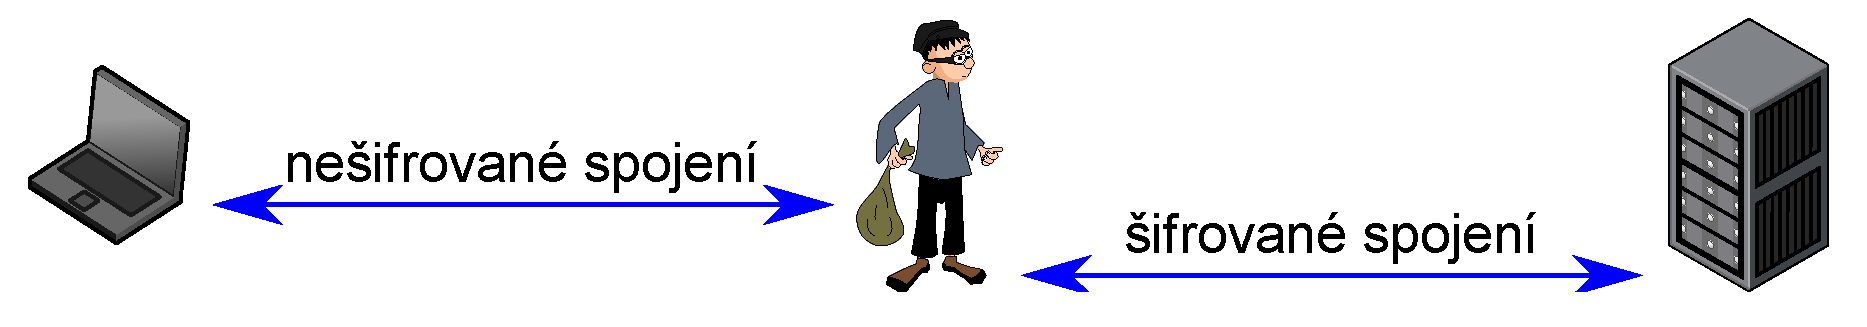
\includegraphics[width=0.9\linewidth]{https_stripping.pdf}
        \caption{Útočník MITM přiměje oběť k přístupu přes HTTP.}
    \end{figure}

    \item HTTP hlavička \textbf{HTTP Strict-Transport-Security} \begin{compactitem}
        \item Na této doméně se vždy šifruje (platí pro všechny porty).
        \item Při HTTP server pošle výzvu, že jakékoliv HTTP požadavky předělat na HTTPS.
    \end{compactitem}
\end{compactitem}

\subsection{Clickjacking}

\begin{compactitem}
    \item Zobrazení několika vrstev prvků přes sebe (neviditelná vrstva).
    \item Uživatel si myslí, že kliká na něco jiného než ve skutečnosti.
    \item Při útoku jsou využívány plovoucí rámce (iframe).
    \item Řešení spočívá v zakázání/omezení zobrazení stránky v iframe.

    \item HTTP hlavička \textbf{X-Frame-Options} \begin{compactitem}
        \item Povoluje/zakazuje/omezuje zobrazení stránky v rámci iframe.
    \end{compactitem}

    \item Hlavička \textbf{Content Security Policy}.
\end{compactitem}

% Pokracovani:
% cas 58:00
